%%%%%%%%%%%%%%%%%%%%%%%%%%%%%%%%%%%%%%%%%
% University/School Laboratory Report
% LaTeX Template
% Version 3.1 (25/3/14)
%
% This template has been downloaded from:
% http://www.LaTeXTemplates.com
%
% Original author:
% Linux and Unix Users Group at Virginia Tech Wiki
% (https://vtluug.org/wiki/Example_LaTeX_chem_lab_report)
%
% License:
% CC BY-NC-SA 3.0 (http://creativecommons.org/licenses/by-nc-sa/3.0/)
%
%%%%%%%%%%%%%%%%%%%%%%%%%%%%%%%%%%%%%%%%%

%----------------------------------------------------------------------------------------
%	PACKAGES AND DOCUMENT CONFIGURATIONS
%----------------------------------------------------------------------------------------

\documentclass{article}
\usepackage[utf8]{inputenc}
\usepackage{appendix}
\usepackage[T1]{fontenc}
\usepackage{siunitx} % Provides the \SI{}{} and \si{} command for typesetting SI units
\usepackage{graphicx} % Required for the inclusion of images
\usepackage{natbib} % Required to change bibliography style to APA
\usepackage{amsmath} % Required for some math elements
\usepackage{caption}
\usepackage{tikz}


\usepackage{float}


\usetikzlibrary{arrows,automata, positioning}

\usepackage{import}

\setlength\parindent{0pt} % Removes all indentation from paragraphs

%----------------------------------------------------------------------------------------
%	DOCUMENT INFORMATION
%----------------------------------------------------------------------------------------

\title{Prova Finale di Reti Logiche} % Title
\author{Montanari Tommaso e Negri Riccardo} % Author name
\date{1 Aprile 2022}

\begin{document}
\maketitle % Insert the title, author and date
\begin{center}
\begin{tabular}{l l l l}
Docente: & Salice Fabio & & \\ 
Studente 1: & Montanari Tommaso & 10661941 & 932673\\
Studente 2: & Negri Riccardo & 10729927 & 936820 
\end{tabular}
\end{center}

% If you wish to include an abstract, uncomment the lines below
% \begin{abstract}
% Abstract text
% \end{abstract}

%----------------------------------------------------------------------------------------
%	SECTION 1
%----------------------------------------------------------------------------------------

\section{Introduzione}

La prova prevede l'implementazione in VHDL di una macchine che opera su una memoria e svolge la seguente operazione.

La macchina deve per prima cosa leggere il primo byte dalla memoria che identifica il numero di parole che sono
state fornite come input, questa informazione è importante per capire quando la macchina deve terminare la lettura.

Dopodiché ogni parola successiva viene tradotta in due parole di memoria che vengono scritte progressivamente in un'altra parte della memoria.

\subsection{Esempio}

\begin{tabular}{c c c}
	Indirizzo & Valore & Codifica binaria \\
	0 & 2 & 0000 0010 \\
	1 & 35 & 0010 0011 \\
	2 & 161 & 1010 0001 \\
\end{tabular}
\\
\\
Questo stato della memoria si traduce nell'input [35, 161] e in questo caso la lunghezza dell'input W=2 quindi mi aspetto una lunghezza dell'output Z=4.
\\
\\
\begin{tabular}{c c c}
	Indirizzo & Valore & Codifica binaria \\
	1000 & 13 & 0000 1101 \\
	1001 & 206 & 1100 1110 \\
	1002 & 97 & 0110 0001 \\
	1003 & 195 & 1100 0011 \\
\end{tabular}
\\
\\
Rappresenta l'output [13, 206, 97, 195] dove [13, 206] sono i numeri che sono stati prodotti dal 35 in ingresso mentre [97, 195] sono ottenuti processando 161

\subsection{Ipotesi Progettuali}
\begin{itemize}
\item {Si utilizza la scheda Artix-7 FPGA xc7a200tfbg484-1}
\item {Ogni byte può contenere numeri da 0 a 255.}
\item {La quantità di numeri in ingresso (W) è contenuta in una parola da un byte quindi anche il numero massimo di parole da tradurre è 255.}
\item {Dato che l'input occupa al massimo 256 byte posso scrivere sui byte successivi quindi l'output parte sempre dal millesimo indirizzo di memoria che sicuramente non contiene l'input}
\end{itemize}




%----------------------------------------------------------------------------------------
%	SECTION 2
%----------------------------------------------------------------------------------------

\section{Architetttura}
Architetttura



%----------------------------------------------------------------------------------------
%	SECTION 3
%----------------------------------------------------------------------------------------

\section{Risultati sperimentali}
\subsection{Sintesi}
Il componente sviluppato è sintetizzabile ed implementabile. 
\begin{figure}[H]
	\centering
	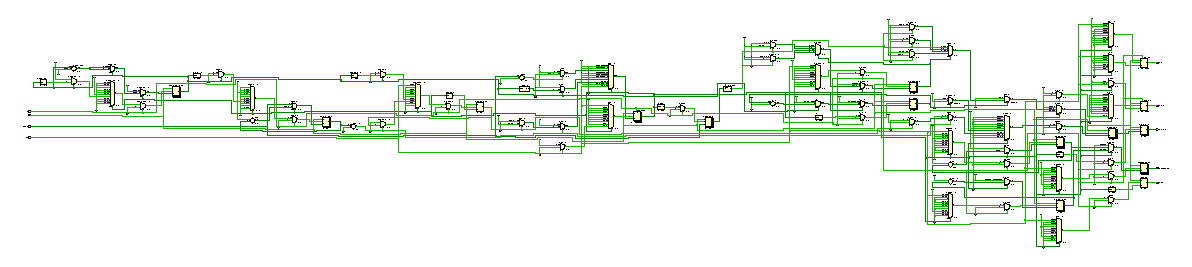
\includegraphics[width=1\textwidth]{schematic.eps}
	\caption{Schema post-sintesi}
\end{figure}
Nella seguente tabella sono indicati i componenti utilizzati nella sintesi.
\begin{center}
	\begin{tabular}{|c|c|c|c|}
		\hline
		Site Type   & Used & Available & Utilization\% \\
		\hline
		LUT as Logic & 117 & 134600 & 0.09 \\
		\hline
		Register as Flip Flop & 95 & 269200  & 0.04\\
		\hline
		F7 Muxes & 1 & 67300 & <0.01\\
		\hline
	\end{tabular}
\end{center}



\subsection{Simulazioni}
Al fine di verificare il corretto funzionamento del componente sono stati eseguiti diversi test bench in simulazioni Behavioural, Post-synthesis functional e Post-synthesis timing. 
Di seguito sono riportati i test significativi effettuati con relativa spiegazione, tempi ottenuti e grafico d'onda.

\subsubsection{Flussi successivi}
Tramite questo test si verifica la correttezza  nel caso di codifica di più flussi uno dopo l'altro. Nel testbench usato vengono codificati tre flussi (senza reset dopo ogni flusso).
\begin{description}
	\item[Behavioural] 21850 ns
	\item[Post-synthesis functional] 22350100 ps
	\item[Post-synthesis timing] 22353714 ps
\end{description}
\begin{figure}[H]
	\centering
	\includegraphics[width=1\textwidth]{Assets/tb1.png}
	\caption{Post-synthesis functional simulation waveform}
\end{figure}

\subsubsection{Reset asincrono}
Tramite questo test si verifica il corretto funzionamento del reset asincrono.
\begin{description}
	\item[Behavioural] 10650 ns
	\item[Post-synthesis functional] 10750100 ps
	\item[Post-synthesis timing] 10753714 ps
\end{description}
\begin{figure}[!htb]
	\centering
	\includegraphics[width=1\textwidth]{Assets/tb2.png}
	\caption{Post-synthesis functional simulation waveform}
\end{figure}

\subsubsection{Sequenza di lunghezza massima}
\paragraph{}Tramite questo test si verifica il corretto funzionamento nel caso di sequenza di ingresso di lunghezza massima: 255 byte.
\begin{description}
	\item[Behavioural] 332450 ns
	\item[Post-synthesis functional] 332550100 ps
	\item[Post-synthesis timing] 332553714 ps
\end{description}
In questo caso non si riporta grafico della forma d'onda perché non è possibile distinguere i valori che i segnali assumono nella vista "fit".
%\begin{figure}[!htb]
%	\centering
%	\includegraphics[width=1\textwidth]{Assets/tb3.png}
%	\caption{Post-synthesis functional simulation waveform}
%\end{figure}

\subsubsection{Sequenza di lunghezza nulla}
Tramite questo test si verifica il corretto funzionamento nel caso di sequenza di ingresso di lunghezza minima: 0 byte.
\begin{description}
	\item[Behavioural] 950 ns
	\item[Post-synthesis functional] 1050100 ps
	\item[Post-synthesis timing] 1053714 ps
\end{description}
\begin{figure}[H]
	\centering
	\includegraphics[width=1\textwidth]{Assets/tb4.png}
	\caption{Post-synthesis functional simulation waveform}
\end{figure}

\subsubsection{Double processing sulla stessa RAM}
Tramite questo test si verifica il corretto funzionamento nel caso di scrittura sulla stessa RAM.
\begin{description}
	\item[Behavioural] 9250 ns
	\item[Post-synthesis functional] 9550100 ps
	\item[Post-synthesis timing] 9553714 ps
\end{description}
\begin{figure}[H]
	\centering
	\includegraphics[width=1\textwidth]{Assets/tb5.png}
	\caption{Post-synthesis functional simulation waveform}
\end{figure}

\subsubsection{Tests con reset}
Test bench, con reset dopo ogni test, che effettua 1000 test (generati casualmente con uno script Python).
\begin{description}
	\item[Behavioural] 172743250 ns
	\item[Post-synthesis functional] 172943150100 ps
	\item[Post-synthesis timing] 172943153714 ps
\end{description}
In questo caso non si riporta grafico della forma d'onda perché non è possibile distinguere i valori che i segnali assumono nella vista "fit".

\subsubsection{Tests senza reset}
Test bench, senza reset dopo ogni test, che effettua 1000 test (generati casualmente con uno script Python).
\begin{description}
	\item[Behavioural] 172543450 ns
	\item[Post-synthesis functional] 172743350100 ps
	\item[Post-synthesis timing] 172743353714 ps
\end{description}
In questo caso non si riporta grafico della forma d'onda perché non è possibile distinguere i valori che i segnali assumono nella vista "fit".

\subsection{Osservazioni}
Osservazioni su tempo di clock minimo.\\
Osservazioni su come reset non genera ritardi(?).

%----------------------------------------------------------------------------------------
%	SECTION 4
%----------------------------------------------------------------------------------------

\section{Conclusioni}


%----------------------------------------------------------------------------------------

\end{document}